\section{Evaluation and Results}
\label{sec:results}

\subsection{Experimental Setup and Evaluation Protocol}
All results are obtained from PX4 Software-In-The-Loop (SITL) coupled to a per-vehicle JSBSim fixed-wing flight-dynamics model through a Micro-XRCE-DDS bridge, with the thermal field, stochastic ground events, field-of-view (FOV) sensing, propulsion-energy estimator and finite-state-machine (FSM) autonomy implemented as ROS\,2 nodes. Table~\ref{tab:experimental_campaign} summarises the campaign. Each run is fully seeded and reproducible; the master seed drives the thermal field and the ground-event process. Campaign runs execute a $600$\,s simulated horizon ($900$\,s for the nominal case study) at real-time lockstep, with the battery capacity scaled so the complete energy-aware FSM cycle executes within the horizon. Reported durations are therefore short-horizon framework-execution times, not vehicle-endurance claims, and all energy quantities are propulsion-only (avionics, payload, communication and onboard computing are excluded).

\subsection{Framework Verification}
Table~\ref{tab:framework_verification} reports the verification suite. The PX4 extended Kalman filter (EKF) estimate is compared against the JSBSim flight-dynamics ground truth relayed through \texttt{HIL\_STATE\_QUATERNION}; Fig.~\ref{fig:px4_jsbsim_verification} shows altitude, ground-speed and attitude comparisons with their error traces and the shaded initialization window. After the documented $20$\,s estimator-convergence window is excluded, the mean post-initialization root-mean-square errors are 1.90\,m (position), 1.90\,m (altitude), 0.28\,m/s (velocity), 0.28\,m/s (vertical speed) and 0.81$^\circ$ (attitude), with no post-initialization gross outliers. Position RMSE is the three-dimensional local-NED position-vector error $\sqrt{e_x^2+e_y^2+e_z^2}$; altitude RMSE is the vertical ($-z$) error; velocity RMSE is the three-dimensional NED velocity-vector error; vertical-speed RMSE is the $v_z$ error; and attitude RMSE is the magnitude of the roll/pitch/yaw error vector. Per-component acceptance thresholds (position $\leq5$\,m, altitude $\leq5$\,m, velocity $\leq2$\,m/s, vertical speed $\leq2$\,m/s, attitude $\leq10^\circ$) are listed in Table~\ref{tab:framework_verification} and all are met. The verification status is therefore \texttt{PASS\_WITH\_DOCUMENTED\_STARTUP\_TRANSIENTS}. ROS\,2 namespace isolation is established at the message level: each UAV owns a unique \texttt{px4\_$i$} namespace and source identifier with consistent topic ownership, and no node received a message from an incorrect namespace. Command routing, FOV detection, event-state correctness, thermal-parameter validity, SOC/log synchronization, landing-state validity and log completeness also pass.

\subsection{Coverage-Path and Executed-Trajectory Analysis}
Fig.~\ref{fig:planned_executed_trajectories} shows the planned partitioned route (panel a) and the executed multi-UAV trajectories (panel b), including thermal footprints, thermal-exploitation segments with entry/exit markers, investigated high-priority (HP) event loiters, glide-return and landing segments. Table~\ref{tab:coverage_path_comparison} compares the selected route against standard coverage strategies using the actual FOV ground footprint. The selected partitioned route has a total length of 23.3\,km with 63\,\% FOV coverage; the lawnmower and boustrophedon strategies achieve higher coverage at the cost of longer paths. The selected route is reasonable for the scenario but is \emph{not} claimed to be optimal.

\subsection{Reduced-Framework Baseline Comparison}
Table~\ref{tab:reduced_framework_baselines} and Fig.~\ref{fig:reduced_framework_baselines} compare the full framework against five reduced configurations over five matched seeds. Improvements and degradations are interpreted separately. Disabling event response removes HP-event investigation entirely while preserving more energy; disabling soaring removes thermalling and its energy benefit but can increase route completion because the vehicle no longer diverts to exploit lift; the non-energy-aware FSM produces a lower final SOC than the full framework; and the simplified-battery model changes the SOC interpretation. Each ablation produces the expected capability-specific trade-off rather than a uniform degradation.

\subsection{Propulsion-Energy Assessment}
Fig.~\ref{fig:propulsion_energy_assessment} presents the propulsion-only energy budget by FSM mode (panel a), SOC trajectories coloured by mode (panel b), and the online state-dependent estimator against a constant-power model and the PX4 battery estimate (panel c). Thermal-exploitation energy is reported as propulsion energy avoided relative to powered cruise. No external real-flight reference is available, and no experimental real-flight validation is claimed.

\subsection{Thermal-Field Sensitivity Analysis}
Fig.~\ref{fig:thermal_field_sensitivity} reports thermal encounters per UAV, thermalling duration, propulsion-energy saving relative to powered cruise, and final SOC across low, nominal and high thermal conditions (five matched seeds each). Thermalling duration rises from 12\,s (low) to 944\,s (high), and the propulsion-energy saving rises from 0.1\,Wh to 7.1\,Wh, a monotonic response. Fig.~\ref{fig:thermal_interaction_trace} shows a representative exploitation segment: the UAV circles within the active thermal footprint while altitude increases and propulsion energy remains essentially flat (motor-off soaring).

\subsection{Ground-Event Sensitivity Analysis}
Fig.~\ref{fig:ground_event_sensitivity} reports HP-event outcomes and investigation latency across event loads. HP investigation percentage is 13\,\%, 26\,\% and 18\,\% at low, nominal and high load respectively; investigation percentage varies non-monotonically with workload. Panel (b) reports investigation latency with the number of investigated events annotated for every condition. The low-load latency value rests on only a few investigated events and is descriptive rather than statistically representative; mean, median and a one-standard-deviation interval (clamped at zero) are shown only where at least two investigated events are available. Outcomes are reported as counts and percentages rather than rates.

\subsection{Repeated Stochastic Evaluation}
Table~\ref{tab:stochastic_results} and Fig.~\ref{fig:repeated_stochastic_summary} summarise 20 seeded runs of the full framework. Route completion is 53.8\,\% ($\pm$6.0\,\% at 95\,\% confidence), final SOC 20.9\,\%, HP investigation 26.0\,\%, and detected-event percentage 29.2\,\%, with 0.00 process failures per run. We report valid scenario termination rather than an ambiguous mission-completion metric.

\subsection{Scalability and Resource-Overhead Analysis}
Table~\ref{tab:scalability_overhead} and Fig.~\ref{fig:scalability_overhead} report resource overhead at 6, 12 and 24 UAVs (three seeds each), with the denominator fixed to the requested fleet size. After correcting an offboard-port assignment defect that previously prevented vehicles with two-digit identifiers from arming, arming success is 100\,\% at all three fleet sizes. CPU utilisation rises from 24.5\,\% at 6 UAVs to 71.7\,\% at 24 UAVs while the real-time factor stays near unity. The framework maintained full arming and near-real-time execution at 24 UAVs, although MAVLink timeout frequency increased and remains a communication-overhead limitation: no MAVLink timeouts occurred at 6 or 12 UAVs, whereas at 24 UAVs the timeouts totalled 73 across 3 runs (24.3 per run, 1.01 per UAV, 0.51 per UAV-minute). These were heartbeat-telemetry gaps from which the links recovered; all 24 vehicles armed and produced complete trajectory logs, no commands were permanently lost, and no process failures occurred, so mission execution and process stability were not observably affected. The split between startup and in-mission timeouts was not individually timestamped (NR), and the per-message drop rate was not instrumented (NR).

\subsection{Landing-Cycle Validation}
Table~\ref{tab:landing_validation} and Fig.~\ref{fig:landing_cycle_validation} report 6 landing trials from distinct approach positions. Touchdown success requires a spatial landing-zone condition (within a 100\,m radius of the landing point) in addition to low altitude and ground speed. Landing-state entry and approach completion are 100\,\% and 100\,\%; landing-zone success is 83\,\%, touchdown success 67\,\% and landing completion 67\,\%, with a mean final altitude error of 1.93\,m, mean cross-track error 55\,m and a maximum sustained descent rate of 2.72\,m/s computed over a fixed time window (rather than instantaneous derivative spikes). No command rejections or MAVLink timeouts occurred. Full landing completion was achieved in 4 of 6 trials (66.7\,\%); landing was therefore not fully reliable across all vehicles. The 100\,m landing-zone radius is an acceptance region for autonomous descent and arrival (an operational safety area), not a prepared landing field. Accordingly, this experiment evaluates autonomous descent and arrival within an operational landing zone; it does not evaluate precision runway touchdown, and the result is not described as precision landing.

\subsection{Summary of Findings}
The framework executes the coupled fixed-wing, thermal, ground-event, sensing, propulsion-energy and multi-UAV pipeline reproducibly. Verification shows the PX4 estimate tracks the JSBSim ground truth within documented bounds, and the component ablations produce the expected capability-specific trade-offs. Thermal sensitivity exhibits the expected monotonic trends, while event investigation percentage varies non-monotonically with workload. The repeated-seed experiments quantify the variability and confidence intervals of the principal outcomes rather than implying uniformly low variability: route completion, thermalling duration and event-investigation latency all show substantial run-to-run spread (the low-load latency in particular rests on few investigated events). The framework scales to 24 vehicles with full arming success and near-real-time execution, although MAVLink timeout frequency increases at 24 UAVs and remains a communication-overhead limitation. The landing cycle is validated against a spatial landing-zone criterion with full landing completion in 4 of 6 trials. No optimality or real-flight-validity claims are made.

\begin{figure*}[t]
\centering
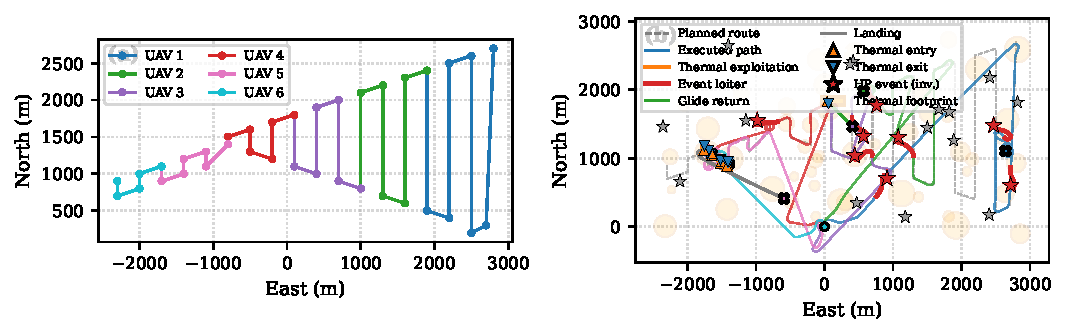
\includegraphics[width=0.95\linewidth]{figures/planned_executed_trajectories.pdf}
\caption{Planned partitioned coverage route (a) and executed multi-UAV trajectories (b) for the nominal case study, with thermal footprints, thermal entry/exit, event loiters, glide-return and landing segments.}
\label{fig:planned_executed_trajectories}
\end{figure*}

\begin{figure*}[t]
\centering
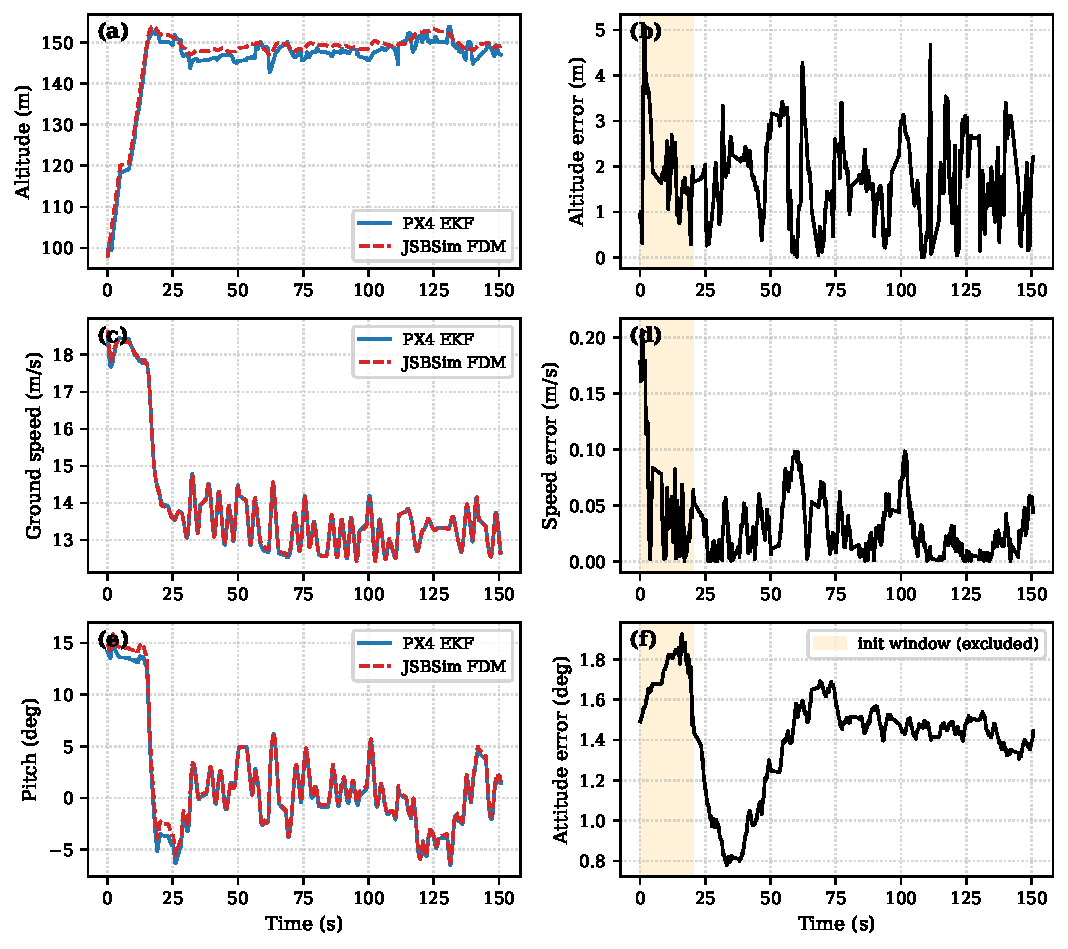
\includegraphics[width=0.95\linewidth]{figures/px4_jsbsim_verification.pdf}
\caption{PX4-EKF versus JSBSim-FDM comparison: altitude (a,b), ground speed (c,d) and attitude (e,f) with error traces. The shaded interval is the excluded initialization window; status PASS\_WITH\_DOCUMENTED\_STARTUP\_TRANSIENTS.}
\label{fig:px4_jsbsim_verification}
\end{figure*}

\begin{figure*}[t]
\centering

\includegraphics[width=0.95\linewidth]{figures/reduced_framework_baselines.pdf}
\caption{Reduced-framework baselines: final SOC (a), propulsion energy (b), HP-event investigation percentage (c) and thermalling duration (d); bars show mean and standard deviation over matched seeds.}
\label{fig:reduced_framework_baselines}
\end{figure*}

\begin{figure*}[t]
\centering
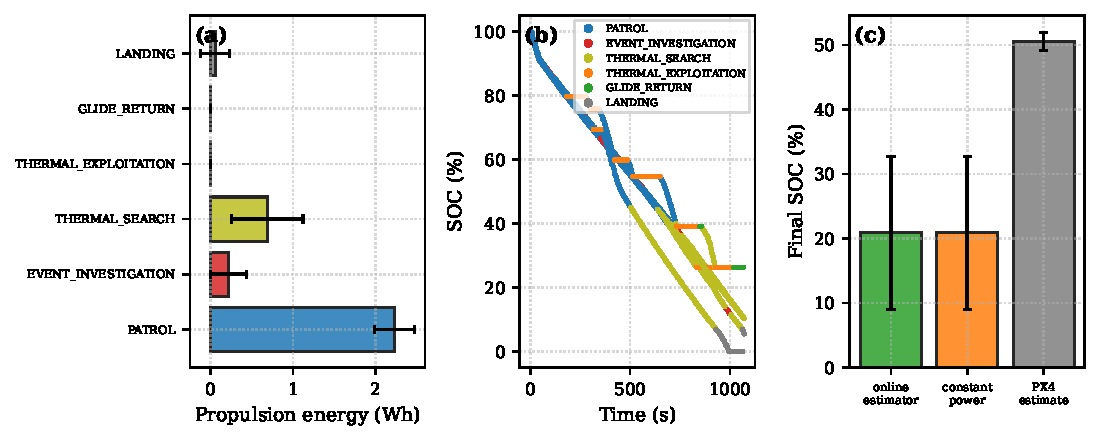
\includegraphics[width=0.95\linewidth]{figures/propulsion_energy_assessment.pdf}
\caption{Propulsion-only energy assessment: energy by FSM mode (a), SOC trajectories by mode (b), and online estimator versus constant-power model and PX4 estimate (c).}
\label{fig:propulsion_energy_assessment}
\end{figure*}

\begin{figure*}[t]
\centering
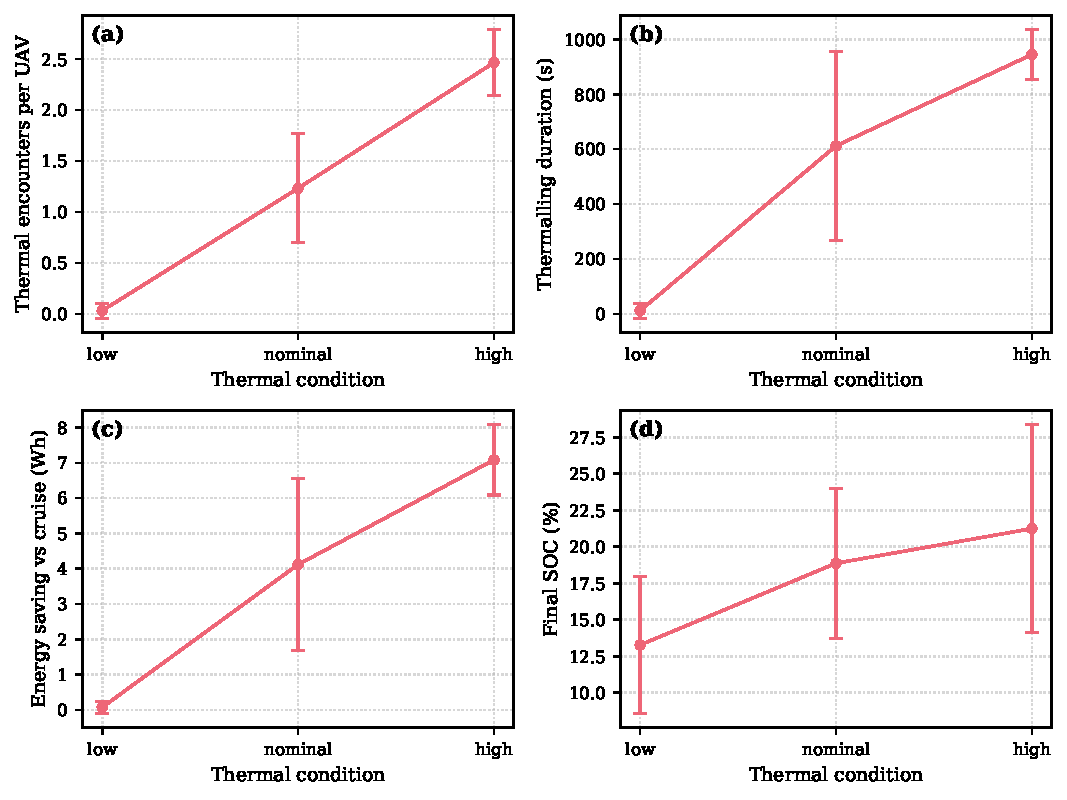
\includegraphics[width=0.95\linewidth]{figures/thermal_field_sensitivity.pdf}
\caption{Thermal-field sensitivity across low, nominal and high conditions: encounters per UAV (a), thermalling duration (b), energy saving relative to cruise (c) and final SOC (d); error bars show standard deviation.}
\label{fig:thermal_field_sensitivity}
\end{figure*}

\begin{figure*}[t]
\centering
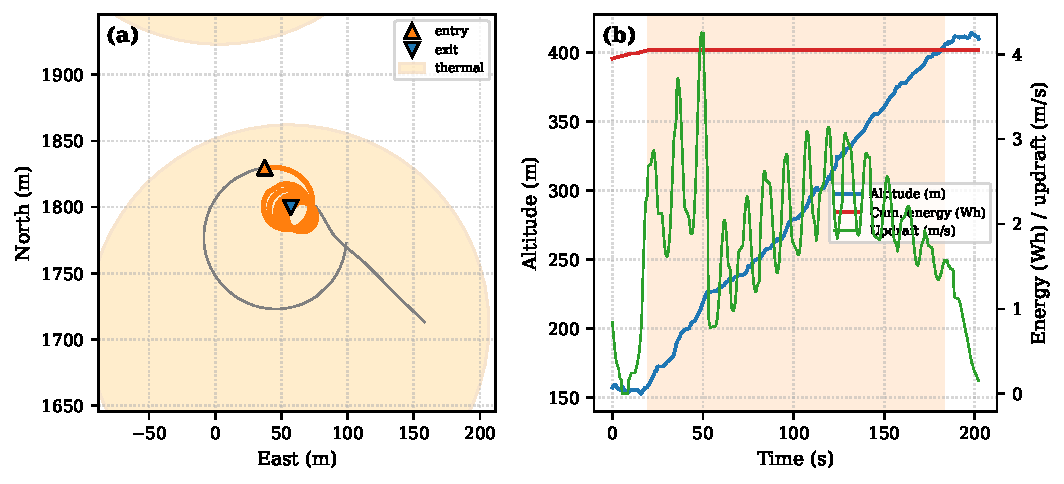
\includegraphics[width=0.95\linewidth]{figures/thermal_interaction_trace.pdf}
\caption{Representative thermal interaction: UAV trajectory inside the active thermal footprint (a) and altitude, updraft and cumulative propulsion energy versus time (b), with the thermal-exploitation interval shaded.}
\label{fig:thermal_interaction_trace}
\end{figure*}

\begin{figure*}[t]
\centering
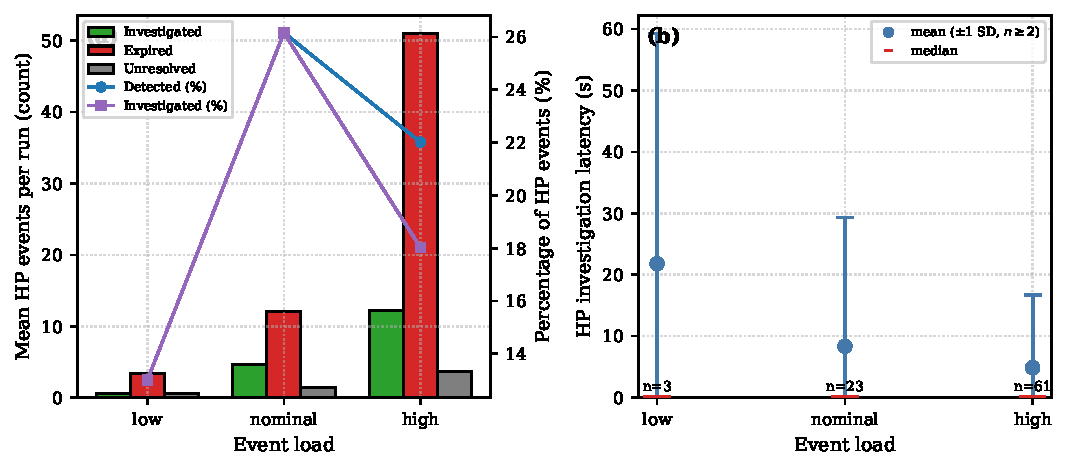
\includegraphics[width=0.95\linewidth]{figures/ground_event_sensitivity.pdf}
\caption{Ground-event sensitivity: mean HP-event outcomes and detection/investigation percentages by load (a) and investigation latency (b). The sample count $n$ of investigated events is annotated for every condition; mean, median and a one-standard-deviation interval (clamped at zero) are shown only for $n\geq2$. The low-load latency is descriptive, resting on few investigated events, and is not statistically representative.}
\label{fig:ground_event_sensitivity}
\end{figure*}

\begin{figure*}[t]
\centering

\includegraphics[width=0.95\linewidth]{figures/repeated_stochastic_summary.pdf}
\caption{Repeated stochastic evaluation over 20 seeds: route completion (a), final SOC (b), thermal encounters (c), thermalling duration (d), HP investigation (e) and detected events (f). Boxplots show median and quartiles; diamonds mark the mean.}
\label{fig:repeated_stochastic_summary}
\end{figure*}

\begin{figure*}[t]
\centering

\includegraphics[width=0.95\linewidth]{figures/scalability_overhead.pdf}
\caption{Scalability and resource overhead versus fleet size: CPU (a), memory (b), real-time factor (c) and ROS\,2 latency (d); error bars span repeated runs.}
\label{fig:scalability_overhead}
\end{figure*}

\begin{figure*}[t]
\centering
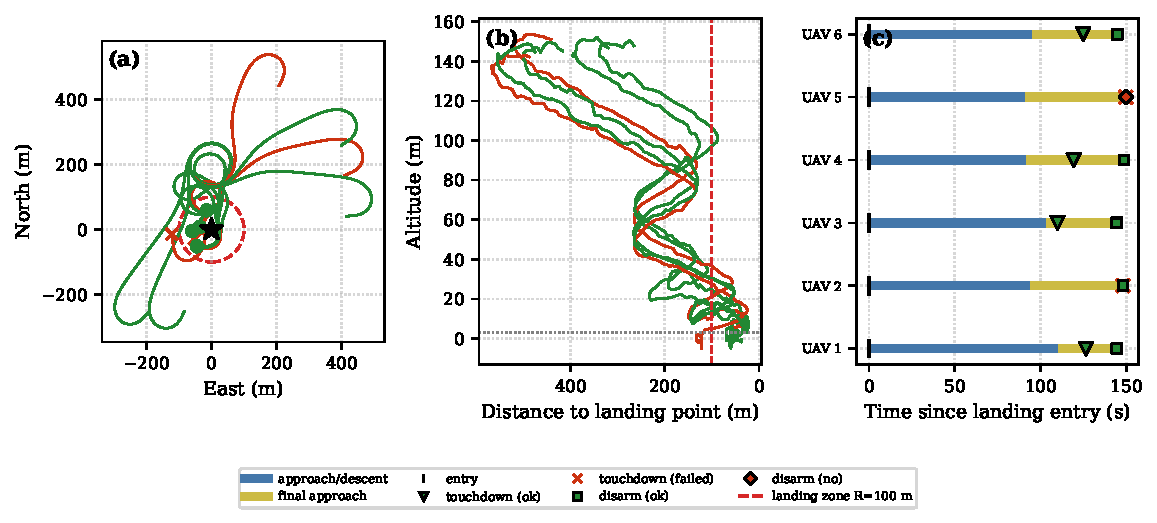
\includegraphics[width=0.95\linewidth]{figures/landing_cycle_validation.pdf}
\caption{Landing-cycle validation: ground tracks with the landing zone (a), altitude versus distance to the landing point (b), and per-UAV landing-subphase timeline (c) showing approach/descent and final-approach phases with entry, touchdown and disarm markers. Green/red distinguish successful and failed touchdown and disarm. Full landing completion was achieved in 4 of 6 trials.}
\label{fig:landing_cycle_validation}
\end{figure*}

\begin{table*}[t]
\centering
\small
\caption{Experimental campaign matrix. New runs are newly executed; reused runs are shared seeds counted once and re-analysed (full-framework baseline and nominal sensitivity conditions reuse stochastic seeds 42--46). Landing validation is a single six-UAV simulation yielding six vehicle-level trials.}
\label{tab:experimental_campaign}
\resizebox{\textwidth}{!}{%
\begin{tabular}{lccccccl}
\toprule
Experiment & Fleet size & New runs & Reused runs & Total analysed runs & Seeds & Horizon & Purpose \\
\midrule
Nominal case study & 6 & 1 & 0 & 1 & 42 & 900 s & End-to-end demonstration \\
Repeated stochastic & 6 & 20 & 0 & 20 & 42--61 & 600 s & Distributional statistics \\
Reduced baselines & 6 & 25 & 5 & 30 & 42--46 & 600 s & 5 ablations x 5 seeds; full-framework reuses stochastic 42--46 \\
Thermal sensitivity & 6 & 10 & 5 & 15 & 42--46 & 600 s & low/high (10 new); nominal reuses stochastic 42--46 \\
Event sensitivity & 6 & 10 & 5 & 15 & 42--46 & 600 s & low/high (10 new); nominal reuses stochastic 42--46 \\
Scalability & 6/12/24 & 9 & 0 & 9 & 101--103 & 120 s & Resource overhead (3 seeds/size) \\
PX4--JSBSim verification & 6 & 1 & 0 & 1 & -- & 150 s & EKF vs FDM consistency capture \\
Landing validation & 6 & 1 & 0 & 1 & 201 & 300 s & one six-UAV simulation = six vehicle-level landing trials \\
\bottomrule
\end{tabular}}
\end{table*}

\begin{table*}[t]
\centering
\small
\caption{Framework-verification summary. The PX4--JSBSim row reports the final post-initialization result only.}
\label{tab:framework_verification}
\resizebox{\textwidth}{!}{%
\begin{tabular}{lllrll}
\toprule
Verification check & Metric & Acceptance threshold & Samples & Result & Notes \\
\midrule
PX4-EKF vs JSBSim-FDM & pos(3D NED)/alt/vel/vspeed/att RMSE & 5 m / 5 m / 2 (m/s) / 2 (m/s) / 10 deg & 4482 & PASS\_WITH\_DOCUMENTED\_STARTUP\_TRANSIENTS & means 1.90 m / 1.90 m / 0.28 / 0.28 (m/s) / 0.81 deg; post-init, 20 s init window excluded \\
ROS 2 namespace isolation & consistency check & 0 failures & 441 & PASS & unique px4\textbackslash{}\_$i$ namespace + source ID per UAV; 0 messages from an incorrect namespace \\
MAVSDK command routing & consistency check & 0 failures & 126 & PASS & one connection per UAV \\
FOV detection correctness & consistency check & 0 failures & 33414 & PASS & slant range vs trajectory \\
Event-state correctness & consistency check & 0 failures & 1017 & PASS & lifecycle ordering + priority \\
Thermal-parameter validity & consistency check & 0 failures & 778588 & PASS & within configured bounds \\
SOC/log synchronization & consistency check & 0 failures & 174773 & PASS & SOC monotonic in [0,100] \\
Landing-state validity & consistency check & 0 failures & 19 & PASS & descending landing trajectory \\
Log completeness & consistency check & 0 failures & 210 & PASS & all artefacts present \\
\bottomrule
\end{tabular}}
\end{table*}

\begin{table*}[t]
\centering
\small
\caption{Coverage-path comparison (geometric, FOV-based). The selected route is reasonable but is not claimed optimal.}
\label{tab:coverage_path_comparison}
\resizebox{\textwidth}{!}{%
\begin{tabular}{lrrrrrrr}
\toprule
Coverage strategy & Total length (km) & Mean per UAV (km) & FOV coverage (\%) & Uncovered area (sq km) & Overlap (\%) & Turns & Imbalance \\
\midrule
Selected & 23.29 & 3.88 & 62.9 & 3.36 & 19.5 & 29 & 1.49 \\
North-South lawnmower & 35.87 & 5.98 & 84.9 & 1.36 & 10.6 & 34 & 0.43 \\
East-West lawnmower & 35.19 & 5.86 & 83.4 & 1.50 & 7.5 & 14 & 0.75 \\
Boustrophedon & 37.32 & 6.22 & 85.6 & 1.30 & 13.8 & 34 & 0.39 \\
Spiral/inward coverage & 42.71 & 6.52 & 83.8 & 1.46 & 18.2 & 17 & 0.36 \\
\bottomrule
\end{tabular}}
\end{table*}

\begin{table*}[t]
\centering
\small
\caption{Reduced-framework baseline comparison (mean and standard deviation over 5 matched seeds; reported as mean (std)).}
\label{tab:reduced_framework_baselines}
\resizebox{\textwidth}{!}{%
\begin{tabular}{lrrrrrrr}
\toprule
Configuration & Final SOC (\%) & Energy (Wh) & Route compl. (\%) & HP inv. (\%) & HP unres. (\%) & Thermalling (s) & Proc. fail \\
\midrule
Full framework & 18.5 (4.1) & 19.8 (1.3) & 60.4 (7.2) & 25.8 (3.3) & 1.9 (3.2) & 483.0 (411.4) & 0.0 (0.0) \\
No thermal & 11.7 (4.8) & 21.5 (1.6) & 86.7 (1.1) & 29.8 (10.4) & 4.8 (5.0) & 0.0 (0.0) & 0.0 (0.0) \\
No event response & 22.2 (6.4) & 19.8 (4.1) & 57.6 (16.6) & 0.0 (0.0) & 7.6 (7.4) & 610.0 (374.0) & 0.0 (0.0) \\
Non-energy-aware FSM & 14.6 (4.5) & 20.5 (1.2) & 79.0 (10.2) & 28.5 (6.9) & 7.6 (7.4) & 470.3 (403.6) & 0.0 (0.0) \\
Simplified battery & 0.0 (0.0) & 51.8 (1.3) & 6.2 (2.1) & 9.1 (7.4) & 7.6 (7.4) & 214.8 (86.9) & 0.0 (0.0) \\
Coverage only & 13.4 (1.3) & 21.0 (0.6) & 86.7 (1.1) & 0.0 (0.0) & 7.6 (7.4) & 0.0 (0.0) & 0.0 (0.0) \\
\bottomrule
\end{tabular}}
\end{table*}

\begin{table*}[t]
\centering
\small
\caption{Repeated stochastic evaluation across 20 seeds (95\% CI = half-width).}
\label{tab:stochastic_results}
\resizebox{\textwidth}{!}{%
\begin{tabular}{lrrrrrr}
\toprule
Metric & Mean & Std & Median & Min & Max & 95\% CI \\
\midrule
Execution duration (s) & 714.25 & 1.59 & 714.17 & 710.34 & 717.03 & 0.69 \\
Route completion (\%) & 53.80 & 13.64 & 55.95 & 30.95 & 73.51 & 5.98 \\
Valid scenario termination (\%) & 85.83 & 16.47 & 83.33 & 50.00 & 100.00 & 7.22 \\
Final SOC (\%) & 20.85 & 5.13 & 21.45 & 9.52 & 30.47 & 2.25 \\
Propulsion energy (Wh) & 19.14 & 1.44 & 18.98 & 16.68 & 22.78 & 0.63 \\
Thermal encounters & 9.20 & 4.94 & 9.00 & 2.00 & 22.00 & 2.16 \\
Thermalling duration (s) & 706.85 & 308.31 & 719.22 & 155.94 & 1157.50 & 135.12 \\
Thermal altitude gain (m) & 154.39 & 45.44 & 143.52 & 79.37 & 236.80 & 19.91 \\
Detected events (\%) & 29.21 & 6.25 & 29.94 & 15.38 & 40.00 & 2.74 \\
HP investigated (\%) & 26.04 & 7.10 & 26.38 & 13.64 & 45.45 & 3.11 \\
HP expired (\%) & 66.67 & 7.93 & 68.47 & 45.45 & 76.19 & 3.48 \\
HP unresolved (\%) & 7.29 & 6.36 & 5.90 & 0.00 & 20.00 & 2.79 \\
HP investigation latency (s) & 3.63 & 6.64 & 0.44 & 0.13 & 26.78 & 2.91 \\
Process failures & 0.00 & 0.00 & 0.00 & 0.00 & 0.00 & 0.00 \\
MAVLink timeouts & 0.00 & 0.00 & 0.00 & 0.00 & 0.00 & 0.00 \\
\bottomrule
\end{tabular}}
\end{table*}

\begin{table*}[t]
\centering
\small
\caption{Scalability and resource overhead (3 seeds per fleet size). Denominator is the requested fleet size. Message-drop rate was not instrumented (NR). MAVLink timeouts are detailed in the timeout analysis.}
\label{tab:scalability_overhead}
\resizebox{\textwidth}{!}{%
\begin{tabular}{lrrrrrrrrrr}
\toprule
Fleet & Armed & Arming (\%) & CPU (\%) & Memory (\%) & RTF & Latency (ms) & Drop rate & MAVLink TO & Proc. fail & Log (MB) \\
\midrule
6 UAVs & 6 & 100 & 24.5 & 22.2 & 1.01 & 5.2 & NR & 0.0 & 0.0 & 3 \\
12 UAVs & 12 & 100 & 44.8 & 23.8 & 1.01 & 7.6 & NR & 0.0 & 0.0 & 7 \\
24 UAVs & 24 & 100 & 71.7 & 28.2 & 1.00 & 17.5 & NR & 24.3 & 0.0 & 13 \\
\bottomrule
\end{tabular}}
\end{table*}

\begin{table*}[t]
\centering
\small
\caption{Landing-cycle outcomes. Touchdown requires the spatial landing-zone condition in addition to low altitude and ground speed.}
\label{tab:landing_validation}
\resizebox{\textwidth}{!}{%
\begin{tabular}{lr}
\toprule
Metric & Value \\
\midrule
Number of trials & 6 \\
Landing-zone radius (m) & 100 \\
Landing-state entry rate (\%) & 100.0 \\
Approach completion rate (\%) & 100.0 \\
Landing-zone success rate (\%) & 83.3 \\
Touchdown success rate (\%) & 66.7 \\
Disarm success rate (\%) & 83.3 \\
Landing completion rate (\%) & 66.7 \\
Mean landing duration (s) & 146.7 \\
Mean final horizontal error (m) & 67.9 \\
Mean cross-track error (m) & 54.6 \\
Mean final altitude error (m) & 1.93 \\
Mean descent rate (m/s) & 1.14 \\
Max sustained descent rate (m/s) & 2.72 \\
Command rejections & 0 \\
MAVLink timeouts & 0 \\
\bottomrule
\end{tabular}}
\end{table*}


